\documentclass{standalone}

\usepackage{tikz}
\usepackage{tkz-euclide}
\usetikzlibrary{calc}
\usetikzlibrary{positioning}
\usetikzlibrary{arrows.meta}

\definecolor{myblue}{rgb}{0.0,0.5,0.8}

\usepackage{times}

\begin{document}
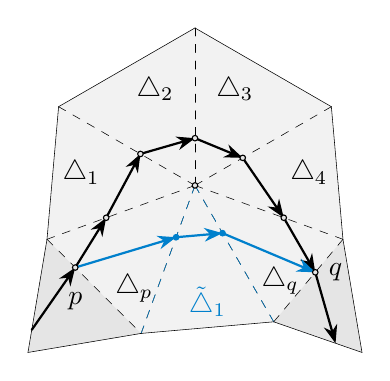
\begin{tikzpicture}[%
  >={Stealth[scale=1.0]},
  scale=2.0,
]

  \tkzDefPoint(0.0, 0.0){v0}

  \tkzDefPointOnCircle[R = center v0 angle 30 radius 1]\tkzGetPoint{v1}
  \tkzDefPointOnCircle[R = center v0 angle 90 radius 1]\tkzGetPoint{v2}
  \tkzDefPointOnCircle[R = center v0 angle 150 radius 1]\tkzGetPoint{v3}
  \tkzDefPointOnCircle[R = center v0 angle 200 radius 1]\tkzGetPoint{v4}
  \tkzDefPointOnCircle[R = center v0 angle 250 radius 1]\tkzGetPoint{v5}
  \tkzDefPointOnCircle[R = center v0 angle -60 radius 1]\tkzGetPoint{v6}
  \tkzDefPointOnCircle[R = center v0 angle -20 radius 1]\tkzGetPoint{v7}

  \tkzDefPointOnCircle[R = center v0 angle -135 radius 1.5]\tkzGetPoint{p}
  \tkzDefPointOnCircle[R = center v0 angle -45 radius 1.5]\tkzGetPoint{q}

  \tkzDefPointOnLine[pos = 0.8](v4,p)\tkzGetPoint{ep}
  \tkzDefPointOnLine[pos = 0.3](v4,v5)\tkzGetPoint{e0}
  \tkzDefPointOnLine[pos = 0.6](v0,v4)\tkzGetPoint{e1}
  \tkzDefPointOnLine[pos = 0.4](v0,v3)\tkzGetPoint{e2}
  \tkzDefPointOnLine[pos = 0.3](v0,v2)\tkzGetPoint{e3}
  \tkzDefPointOnLine[pos = 0.35](v0,v1)\tkzGetPoint{e4}
  \tkzDefPointOnLine[pos = 0.6](v0,v7)\tkzGetPoint{e5}
  \tkzDefPointOnLine[pos = 0.6](v6,v7)\tkzGetPoint{e6}
  \tkzDefPointOnLine[pos = 0.7](v6,q)\tkzGetPoint{eq}

  \tkzDefPointOnLine[pos = 0.35](v0,v5)\tkzGetPoint{r1}
  \tkzDefPointOnLine[pos = 0.35](v0,v6)\tkzGetPoint{r2}

  \tkzFillPolygon[color=black!5](v0,v1,v2)
  \tkzFillPolygon[color=black!5](v0,v2,v3)
  \tkzFillPolygon[color=black!5](v0,v3,v4)
  \tkzFillPolygon[color=black!5](v0,v4,v5)
  \tkzFillPolygon[color=black!5](v0,v5,v6)
  \tkzFillPolygon[color=black!5](v0,v6,v7)
  \tkzFillPolygon[color=black!5](v0,v7,v1)
  \tkzFillPolygon[color=black!10](p,v4,v5)
  \tkzFillPolygon[color=black!10](q,v6,v7)


  % \tkzDrawSegments(v0,v1 v0,v2 v0,v3 v0,v4 v0,v5 v0,v6 v0,v7)
  \tkzDrawSegments[dashed](v0,v1 v0,v2 v0,v3 v0,v4 v0,v5 v0,v6 v0,v7 v4,v5 v6,v7)
  \tkzDrawSegments[dashed,myblue](v0,v5 v0,v6)
  \tkzDrawSegments(v1,v2 v2,v3 v3,v4 v5,v6 v7,v1)
  \tkzDrawSegments(p,v4 p,v5 q,v6 q,v7)
  % \tkzDrawPoints(v0,v1,v2,v3,v4,v5,v6,v7,p,q)
  \tkzDrawPoints(v0)

  \tkzDrawSegments[->,thick](ep,e0 e6,eq)
  \tkzDrawSegments[->,thick](e0,e1 e1,e2 e2,e3 e3,e4 e4,e5 e5,e6)
  \tkzDrawSegments[->,thick,myblue](e0,r1 r1,r2 r2,e6)
  \tkzDrawPoints[myblue](r1,r2)
  \tkzDrawPoints(e0,e1,e2,e3,e4,e5,e6)

  \tkzLabelPoint[below=0.2](e0){$p$}
  \tkzLabelPoint[right=0.05](e6){$q$}

  \tkzLabelSegment[below left = 0.1](v0,v5){$\triangle_p$}
  \tkzLabelSegment[right](v3,v4){$\triangle_1$}
  \tkzLabelSegment[below right](v2,v3){$\triangle_2$}
  \tkzLabelSegment[below left](v2,v1){$\triangle_3$}
  \tkzLabelSegment[left](v1,v7){$\triangle_4$}
  \tkzLabelSegment[left](v6,v7){$\triangle_q$}
  \tkzLabelSegment[above,myblue](v5,v6){$\tilde{\triangle}_1$}

\end{tikzpicture}
\end{document}
